% This is file JFM2esam.tex
% first release v1.0, 20th October 1996
%       release v1.01, 29th October 1996
%       release v1.1, 25th June 1997
%       release v2.0, 27th July 2004
%       release v3.0, 16th July 2014
%   (based on JFMsampl.tex v1.3 for LaTeX2.09)
% Copyright (C) 1996, 1997, 2014 Cambridge University Press

\documentclass{jfm}
\usepackage{graphicx}
\usepackage{epstopdf, epsfig}

\newcommand{\mrd}{\mathrm{d}}
\newcommand{\cE}{\mathcal{E}}
\newtheorem{lemma}{Lemma}
\newtheorem{corollary}{Corollary}

\shorttitle{Viscous elastic fracture}
\shortauthor{T. Large, J. Lister and D. Skinner}

\title{Viscous control of shallow elastic fracture}

\author{Tim Large\aff{1},
  John Lister\aff{2},
 \and Dominic Skinner\aff{2}}
  %\corresp{\email{jfm@damtp.cam.ac.uk}}

\affiliation{\aff{1} M.I.T., USA
\aff{2}Department of Applied Mathematics and Theoretical Physics, University of
Cambridge, UK}

\begin{document}

\maketitle

\begin{abstract}
This paper considers the problem of a semi-infinite crack parallel to the
boundary of a half plane, with the crack filled by an incompressible viscous
fluid. 
The dynamics are driven by a bending moment applied to the arm of the crack,
and we look for travelling wave solutions. We examine two models of fracture;
fracture with a single tip, and fracture with a wet tip proceded by a region
of dry fracture.
\end{abstract}

\begin{keywords}
Authors should not enter keywords on the manuscript, as these must be chosen by the 
author during the online submission process and will then be added during the 
typesetting process (see http://journals.cambridge.org/data/
\linebreak[3]relatedlink/jfm-\linebreak[3]keywords.pdf for the full list)
\end{keywords}

\section{Introduction}\label{sec:introduction}
Here we review the literature as well as describe the problem in more detail.
We have the vertical displacement $h$, the horizontal displacement $g$, the
thickness of the arm $l$, and the pressure $p$.
We look for a travelling wave solution (propagating left), with speed $c$.
%
% 
\section{Formulation of problem}\label{sec:formulation_of_problem}
%
%
From lubrication, we have Poiseulle flow in the crack. We obtain
the flux, and conservation of mass as 
\begin{equation}
q = - \frac{1}{12\mu}\frac{\mrd p}{\mrd x}h^3 \, , \qquad
\frac{\partial q}{\partial x} + \frac{\partial h}{\partial t} = 0 \, ,
\end{equation}
which combined gives
\begin{equation}
\frac{\mrd p}{\mrd x} = 12\mu c / h^2 \, .
\end{equation}
Setting $p\to 0$ at $x \to \infty$, we can write this in integral form,
\begin{equation}
p(x) = -\int_x^{\infty} 12\mu c / h(\tilde{x})^2 \mrd \tilde{x} \, .
\end{equation}

From the linear theory of elasticity, due to others who have studied this 
problem, we have
\begin{equation}
\setlength{\arraycolsep}{2pt}
\left[ \begin{array}{c} 
-\sigma_y \\ -\tau_{xy}
\end{array} \right] 
= 
\left[ \begin{array}{c} 
p(x) \\ 0
\end{array} \right]
=\frac{1}{l}  \int_0^{\infty} \mathsfbi{K} \left( \frac{\tilde{x}-x}{l} \right) 
\left[ \begin{array}{c} 
g'(\tilde{x}) \\ h'(\tilde{x})
\end{array} \right]
\mrd \tilde{x} \, ,
\end{equation}
%
where the integral kernel is
\begin{equation}
\setlength{\arraycolsep}{4pt}
\renewcommand{\arraystretch}{1.3}
\mathsfbi{K}(\xi) = \left[
\begin{array}{ccccc}
  K_{11}  &  K_{12}  \\
K_{21} & K_{22} \\
\end{array}  \right] 
%
= \left[
\begin{array}{ccccc}
  \frac{(32-24\xi^2)}{(\xi^2+4)^3}  &  
\frac{(48\xi^2-64)}{\xi(\xi^2+4)^3}  \\[4pt]
-\frac{(16\xi^4+16\xi^2+4)}{\xi(\xi^2+4)^3} & 
-\frac{(32 - 24\xi^2)}{(\xi^2+4)^3} 
\end{array}  \right] \, .
\end{equation}
The boundary conditions near $x=0$ are governed by fracture mechanics
\refstepcounter{equation}
$$
K_I =\lim_{x \to 0} \frac{E}{1-\nu^2} \sqrt{\frac{\upi}{8}} \sqrt{x} \, h'(x)
\, ,\qquad
K_{II} =\lim_{x \to 0} \frac{E}{1-\nu^2} \sqrt{\frac{\upi}{8}} \sqrt{x} \,
g'(x) \, .
\eqno{(\theequation{\mathit{a},\mathit{b}})}
$$
As we go to $x \gg l$, we are looking at the problem of peeling off a thin
strip from an elastic half space. We can then use beam theory approximations,
which give
\refstepcounter{equation}
$$
M(x) = \frac{El^3}{12(1-\nu^2)} \frac{\mrd^2 h}{\mrd x^2} = 
\frac{El^3}{6(1-\nu^2)} \frac{\mrd g}{\mrd x}, \qquad
p = \frac{El^3}{12(1-\nu^2)} h^{(4)}(x) 
\eqno{(\theequation{\mathit{a},\mathit{b}})}\label{eq:by-at-inf}
$$
As $x \to \infty$, $M(x) \to M$, the applied bending moment, so this gives
us boundary conditions on $h''$, $g'$.
%
\subsection{Rescaling}
%
We can define the following dimensionless variables
\begin{equation} 
x = l\xi,  \quad h(x) = \frac{12M(1-\nu^2)}{El}
H(\xi), \quad g(x) = \frac{12M(1-\nu^2)}{El} G(\xi) \, ,
\end{equation}
\begin{equation}
 p = \frac{3M}{\upi l^2} \Pi(\xi), \quad
K_I = Ml^{-3/2} \kappa_I, \quad
K_{II} = Ml^{-3/2} \kappa_{II}, \quad
\lambda = \frac{4\upi \mu  p^* l^3}{M^2} \, .
\end{equation}
With these scalings, the equations become
\begin{equation}
\setlength{\arraycolsep}{2pt}
\left[ \begin{array}{c} 
\Pi \\ 0
\end{array} \right]
= \int_0^{\infty} \mathsfbi{K}(\tilde{\xi} - \xi) 
\left[ \begin{array}{c} 
G'(\tilde{\xi}) \\ H'(\tilde{\xi})
\end{array} \right]
\mrd \tilde{\xi}
\end{equation}
\refstepcounter{equation}
$$
H^2 \frac{\mrd \Pi}{\mrd \xi} = \lambda
\quad \mbox{ or\ } \quad
\Pi(\xi) = -\int_{\xi}^{\infty} \lambda / H(\tilde{\xi})^2 \mrd \tilde{\xi}
%
\eqno{(\theequation{\mathit{a},\mathit{b}})}
\label{eq:govern}
$$
\begin{equation}
\lim_{\xi \to \infty} H'' = 1 , \quad \lim_{\xi \to \infty} G' = \frac{1}{2}
,\quad
\lim_{\xi \to 0} 3\sqrt{2\upi \xi} H' = \kappa_I , 
\quad
\lim_{\xi \to 0} 3\sqrt{2\upi \xi} G' = \kappa_{II} , 
\end{equation}

These shall be the governing equations for the rest of this paper.

The equations of the linear perturbation 
problem:
\begin{equation}
\Pi = \Pi_0 + \cE \Pi_1 + O(\cE), \quad
H = H_0 + \cE H_1 + O(\cE) \quad
\end{equation}
%
\refstepcounter{equation}
$$
\setlength{\arraycolsep}{2pt}
\left[ \begin{array}{c} 
\Pi_1 \\ 0
\end{array} \right]
= \int_0^{\infty} \mathsfbi{K}(\xi - \tilde{\xi}) 
\left[ \begin{array}{c} 
G_1'(\tilde{\xi}) \\ H_1'(\tilde{\xi})
\end{array} \right]
\mrd \tilde{\xi}, \qquad
H_0^2\Pi_1' + 2H_0 H_1 \Pi_0 ' = \lambda_1
\eqno{(\theequation{\mathit{a},\mathit{b}})}\label{eq:lin-pert}
$$
%
\refstepcounter{equation}
$$
H_1''\to 0 \mbox{ as\ } \xi \to \infty, \qquad
H_1 \sim \xi^{s} + \frac{\tilde{A}\lambda_1}{3\lambda_0^{2/3}} \xi^{2/3}
+ \dots \mbox{ as } \xi \to 0
\eqno{(\theequation{\mathit{a},\mathit{b}})}\label{eq:lin-pert-bc}
$$
But these can be made into a more convenient form, by considering instead
$\tilde{\Pi} = \Pi_0 - 3\lambda_0/\lambda_1 \Pi_1$, and similar for 
$\tilde{H}$, $\tilde{G}$. The equations become
\refstepcounter{equation}
$$
\setlength{\arraycolsep}{2pt}
\left[ \begin{array}{c} 
\tilde{\Pi} \\ 0
\end{array} \right]
= \int_0^{\infty} \mathsfbi{K}(\xi - \tilde{\xi}) 
\left[ \begin{array}{c} 
\tilde{G}'(\tilde{\xi}) \\ \tilde{H}'(\tilde{\xi})
\end{array} \right]
\mrd \tilde{\xi}, \qquad
H_0^2\tilde{\Pi}' + 2H_0 \tilde{H} \Pi_0 ' = 0
\eqno{(\theequation{\mathit{a},\mathit{b}})}\label{eq:rescaled-lin-pert}
$$
%
\refstepcounter{equation}
$$
\tilde{H}''\to 1 \mbox{ as\ } \xi \to \infty, \qquad
\tilde{H} \sim -\frac{3\lambda_0}{\lambda_1} \xi^{s} 
+ \dots \mbox{ as } \xi \to 0
\eqno{(\theequation{\mathit{a},\mathit{b}})}\label{eq:rescaled-lin-pert-bc}
$$
%
%
These are the equations for the two tip problem
\refstepcounter{equation}
$$
\setlength{\arraycolsep}{2pt}
\left[ \begin{array}{c} 
\Pi \\ 0
\end{array} \right]
= \int_{-L}^{\infty} \mathsfbi{K}(\tilde{\xi} - \xi) 
\left[ \begin{array}{c} 
G'(\tilde{\xi}) \\ H'(\tilde{\xi})
\end{array} \right]
\mrd \tilde{\xi}, \qquad
\Pi = \int_{\xi}^{\infty} \lambda / H(\tilde{\xi})^2 \mrd \tilde{\xi}
\eqno{(\theequation{\mathit{a},\mathit{b}})}\label{eq:2-govern}
$$
%
\refstepcounter{equation}
$$
\lim_{\xi \to \infty} H'' = 1 , \quad \lim_{\xi \to \infty} G' = \frac{1}{2}
\eqno{(\theequation{\mathit{a},\mathit{b}})}\label{eq:2-bc-inf}
$$
%
\refstepcounter{equation}
$$
\lim_{\xi \to 0} 3\sqrt{2\pi \xi} H' = 0 , 
\quad
\lim_{\xi \to -L} 3\sqrt{2\pi \xi} G' = \kappa_{II}
\eqno{(\theequation{\mathit{a},\mathit{b}})}\label{eq:2-bc-0}
$$
\section{Numerical scheme}\label{sec:numerical_scheme}
%
%%$$
\subsection{Single Tip}
We discretize the problem by taking $n+1$ points $\boldsymbol{\xi} = (\xi_0 =0,
\xi_1 \dots ,\xi_n)$ at which we measure $H'$, $G'$, and $n$ intermediate 
points $\boldsymbol{\zeta} = (\zeta_0, \dots , \zeta_{n-1})$ at which to measure
$\Pi$, so that $\xi_0 < \zeta_0 < \dots < \zeta_{n-1} < \xi_n$.
We work with $\sqrt{\xi}G'(\xi)$,
$\sqrt{\xi}H'(\xi)$ near the tip to avoid singularities.
We define $\boldsymbol{\theta}_G = [\sqrt{\xi_0}G'(\xi_0), \dots , 
\sqrt{\xi_{t-1}} G'(\xi_{t-1}), G'(\xi_t), \dots G'(\xi_n)]$,
$\boldsymbol{\theta}_H =[\sqrt{\xi_0}H'(\xi_0), \dots , 
\sqrt{\xi_{t-1}} H'(\xi_{t-1}), H'(\xi_t), \dots H'(\xi_n)]$, as well as 
$\boldsymbol{\theta} =  [ \boldsymbol{\theta}_G, \boldsymbol{\theta}_H] $,
(where $\sqrt{\xi_0}G'(\xi_0) = \lim_{\xi \to \xi_0} \sqrt{\xi}G'(\xi)$).
Typically $t \approx n/2$ was used. 
The elasticity integral is linear in $G'$, $H'$, and so the discretized 
integration is linear in $\boldsymbol{\theta}$. Such a linear relation
may be written as 
\begin{equation}
[ \Pi(\zeta_{1}) , \dots , \Pi(\zeta_{n-1}), \, \underbrace{0 \, , \, \dots \, 
,\, 0 }_{n-1} \, ] = \mathsfbi{J} \boldsymbol{\theta} \, .
\end{equation}
By imposing $H(0)=0$, and choosing a sensible interpolation,
one can recover $H(\xi_i)$ from $\boldsymbol{\theta}_H$. Therefore,
from the lubrication integral, there exists another expression for 
$[\Pi(\zeta_0), \dots , \Pi(\zeta_{n-1})]$ as some function of 
$\boldsymbol{\theta}_H$. So we can write 
\begin{equation}
[ \Pi(\zeta_{1}) , \dots , \Pi(\zeta_{n-1}), \, \underbrace{0 \, , \, \dots \, 
,\, 0 }_{n-1} \, ] = \mathsfbi{J} \boldsymbol{\theta} = \boldsymbol{f}
(\boldsymbol{\theta}_H) \, ,
\end{equation}
for some function $\boldsymbol{f}$.

Both $G'(\xi_n)$, and $H''(\xi_n)$ are known from our beam theory
asymptotic expansion. But these are linear in $\boldsymbol{\theta}$, as
$G'(\xi_n) = \theta_n$, and 
$H''(\xi_n) \approx (\theta_{2n}-\theta_{2n-1})/(\xi_n-\xi_{n-1}) $, 
Therefore we can 
add another two rows to $\mathsfbi{J}$, so that
\begin{equation}
\mathsfbi{A}\boldsymbol{\theta} = \left[ 
\boldsymbol{f}(\boldsymbol{\theta}),  
G'(\xi_n), H''(\xi_n)\right] \, .
\end{equation}
Where the $\mathsfbi{A}$ is the enlarged matrix. 
This can be solved by Newton's method from quite arbitrary initial guesses.

For $\xi_i < \xi < \xi_{i+1}$, we interpolate as
\begin{equation}
\setlength{\arraycolsep}{1pt}
G'(\xi) = \left\{ \begin{array}{l}  
\xi^{-1/2}(a_i \xi + b_i) \\[4pt]
a_i \xi + b_i
 \end{array}\right., \;\;
H'(\xi) = \left\{ \begin{array}{l}  
\xi^{-1/2}(c_i \xi^{1/2} + d_i) \\[4pt]
c_i \xi + d_i
 \end{array}\right. , \;\;
\mbox{for} \;\; \left\{ \begin{array}{l}  
i<t\\[4pt]
i\geq t
\end{array}\right.
\end{equation}
The choice of interpolating function 
was based on the appearance of the relevant functions.
We will also define $a_n,b_n,c_n,d_n$ for interpolation beyond $\xi_n$.
With this choice of interpolation,
there exist exact closed form expressions for both the lubrication integral,
and the elasticity integral, in terms of the $a_i - d_i$ coefficients.

We therefore want to determine $a_i -d_i$ in terms of $\boldsymbol{\theta}$.
Continuity of $G'$, $H'$ imposes $2(n-1)$ equations. For $G'$ they are 
\begin{equation}
\setlength{\arraycolsep}{1pt}
\begin{array}{rl}
a_i \xi_{i+1} + b_i~ &= a_{i+1} \xi_{i+1} + b_{i+1} = \theta_{i+1},\mbox{ for } i<n,
\,i\neq t -1 \\[4pt]
\xi^{-1/2}(a_{t-1} \xi_t + b_{t-1}) &= a_t \xi_t + b_t = \theta_t,
\end{array}
\end{equation}
with similar equations for $H'$ (accounting for the slightly different 
interpolation). We also have the $2n$ equations following from the definition
of $\boldsymbol{\theta}$, such as $a_i \xi_i + b_i = \theta_i$ for 
$t\leq i \leq n$. 

From our asymptotic expansion 
(via beam theory) we know $\theta_n = G'(\xi_n)$ and $a_n = G''(\xi_n)$. 
Therefore we can write
\begin{equation}
a_n = \frac{G''(\xi_n)}{G'(\xi_n)} \theta_n, \qquad
b_n  = \theta_n - a_n \xi_n = \left( 1 - \frac{G''(\xi_n)}
{G'(\xi_n)} \right) \theta_n
\end{equation}
With $H$, we know that $c_n = H''(\xi_n)$, $c_{n-1} = H''(\xi_{n-1})$, and
so we have that 
\begin{equation}
c_n = \frac{H''(\xi_n)}{H''(\xi_{n-1})} c_{n-1}, \qquad
d_n = -c_n \xi_n + c_{n-1}\xi_n + d_{n-1}
\end{equation}
Therefore, we have enough equations to 
calculate a matrix $\mathsfbi{T}$, so that
\begin{equation}
[a_1, \dots, a_n, b_1, \dots, b_n, c_1, \dots , c_n, d_1, \dots , d_n] = 
\mathsfbi{T} \boldsymbol{\theta}
\end{equation}

Note that we choose a value of $\lambda$, fix the boundary conditions
at $\xi \to \infty$, then solve the problem and subsequently recover
the boundary conditions at $\xi=0$ ($\kappa_I$, $\kappa_{II}$).
This can then be inverted, so that we think of $\lambda = \lambda(\kappa_I)$.
Physically, we know $\kappa_I$, and want to find $\lambda$, but in numerically
solving the problem, it makes more sense to choose $\lambda$ and recover 
$\kappa_I$.

The spacing of the points should reflect that the important 
part of the problem is happening near the tip, and this is where the points
should be concentrated. The spacing that was typically used in numerical 
calculations was 
\begin{equation}
\xi_i = \tan^2( \chi \; i/m ), \quad i=1,\dots,m < n
\end{equation}
where $\chi$ is chosen so that $\tan^2(\chi) = O(10)$, and the remaining points
are added in a geometric progression, so that 
\begin{equation}
\xi_{i+1} = (\xi_m/\xi_{m-1})\xi_{i} , \quad i = m,\dots,n-1
\end{equation}
%
%
\subsection{Linear Perturbation Problem}
%
%
From equation \ref{eq:rescaled-lin-pert-bc}b, we anticipate a 
singularity of the form $\xi^{s-1}$ in $\tilde{H}'$, (we still expect a
$\xi^{-1/2}$ singularity in $\tilde{G}'$). Therefore, the
interpolation used is
\begin{equation}
\setlength{\arraycolsep}{2pt}
\tilde{G}'(\xi) = \left\{ \begin{array}{l}  
\xi^{-1/2}(a_i \xi + b_i) \\[4pt]
a_i \xi + b_i
 \end{array}\right., \quad
\tilde{H}'(\xi) = \left\{ \begin{array}{l}  
\xi^{s-1}(c_i \xi + d_i) \\[4pt]
c_i \xi + d_i
 \end{array}\right. , \quad
\; \mbox{for\ } \left\{ \begin{array}{l}  
i<t\\[4pt]
i\geq t
\end{array}\right.
\end{equation}
Some of the integrals no longer have exact expressions. In this case, they are
calculated by a numerical integration routine. We define 
$\tilde{\boldsymbol{\theta}}$ to be like $\boldsymbol{\theta}$, but with $\tilde{H}'$,
$\tilde{G}'$ instead of $H$, $G$.

The lubrication equation for the linear perturbation problem 
(\ref{eq:rescaled-lin-pert}b) may be written as
\begin{equation}
\tilde{\Pi}(\zeta) = \int_{\zeta}^{\infty} \frac{2\lambda_0 \tilde{H}}{H_0^3} 
\mrd \xi  \, . \label{eq:lin-pert-lub}
\end{equation}
This is linear in $\tilde{H}$, and so in $\tilde{\boldsymbol{\theta}}$.
The integrals that appear were determined numerically.
We end up with a matrix $\mathsfbi{R}$, such that
\begin{equation}
[ \tilde{\Pi}(\zeta_1), \dots \tilde{\Pi}(\zeta_{n-1}) ] = 
\mathsfbi{R} \tilde{\boldsymbol{\theta}}
\end{equation}
Padding out $\mathsfbi{R}$ with zeros, until it is of size $2n\times2n$, we
see that
\begin{equation}
\left( \mathsfbi{A} - \left[ \begin{array}{c} \mathsfbi{R} \\ \boldsymbol{0}
\end{array} \right] \right) \boldsymbol{\theta} = [0 ,\dots ,0, 
\tilde{G}'(\xi_n), \tilde{H}''(\xi_n) ] \label{eq:lin-lub-matrix}
\end{equation}
Since we haven't changed the integral kernel, the  beam theory asymptotics 
remain the same, and together with \ref{eq:lin-pert-lub}, 
we can calculate an asymptotic expression for
$\tilde{H}''(\xi_n)$, $\tilde{G}'(\xi_n)$. Here, we do not need to deploy
Newton's method, as we can simply solve the linear set of equations, 
\ref{eq:lin-lub-matrix}.


\subsection{Double Tip}
In solving the problem of two tips situated at $-L$ and $0$, it is given
that $H = 0$ for $\xi <0$, and thus $H' = 0$ for $\xi <0$. We take $n$ points
to cover $0 \leq \xi < \infty$, and $r$ points to cover $-L \leq \xi < 0$.
we label these points so that
\begin{equation}
\boldsymbol{\xi} = [  \xi_{-r} = -L ,  \xi_{1-r}, \dots , \xi_0 = 0,
\xi_1 , \dots, \xi_n ] .
\end{equation}
We interpolate $G'$ expecting a $\xi^{-1/2}$ singularity at $\xi = -L$, and
$H'$ expecting a $\xi^{-1/2}$ singularity at $\xi = 0$.
We do not 
calculate $\Pi$ for $\xi <0$ (although it is easily done), but just require that
$\sigma_{xy} = 0$ for $\xi < 0$. This provides enough equations for the problem
to be solved as before, with Newton's method. 

Note that we input $-L$ and $\lambda$ and recover $\kappa_I$, $\kappa_{II}$, where 
$\kappa_I$ is measured at $0$. Physically, for $L>0$, we must have
$\kappa_I=0$. Numerically we solve for some $\lambda$, $L$, find $\kappa_I >0$ 
and extrapolate to $\kappa_I=0$.

The spacing of points for $\xi<0$ was chosen so that there was a concentration
of points near $-L$ and near $0$.

%
%
% 
\clearpage
\section{Results}\label{sec:Results}
%
%
%
\subsection{Single tip}
Start off with some of the basic graphs showing $H'$,$G'$, and $\Pi$ against
$\xi$.
\begin{figure}
  \centerline{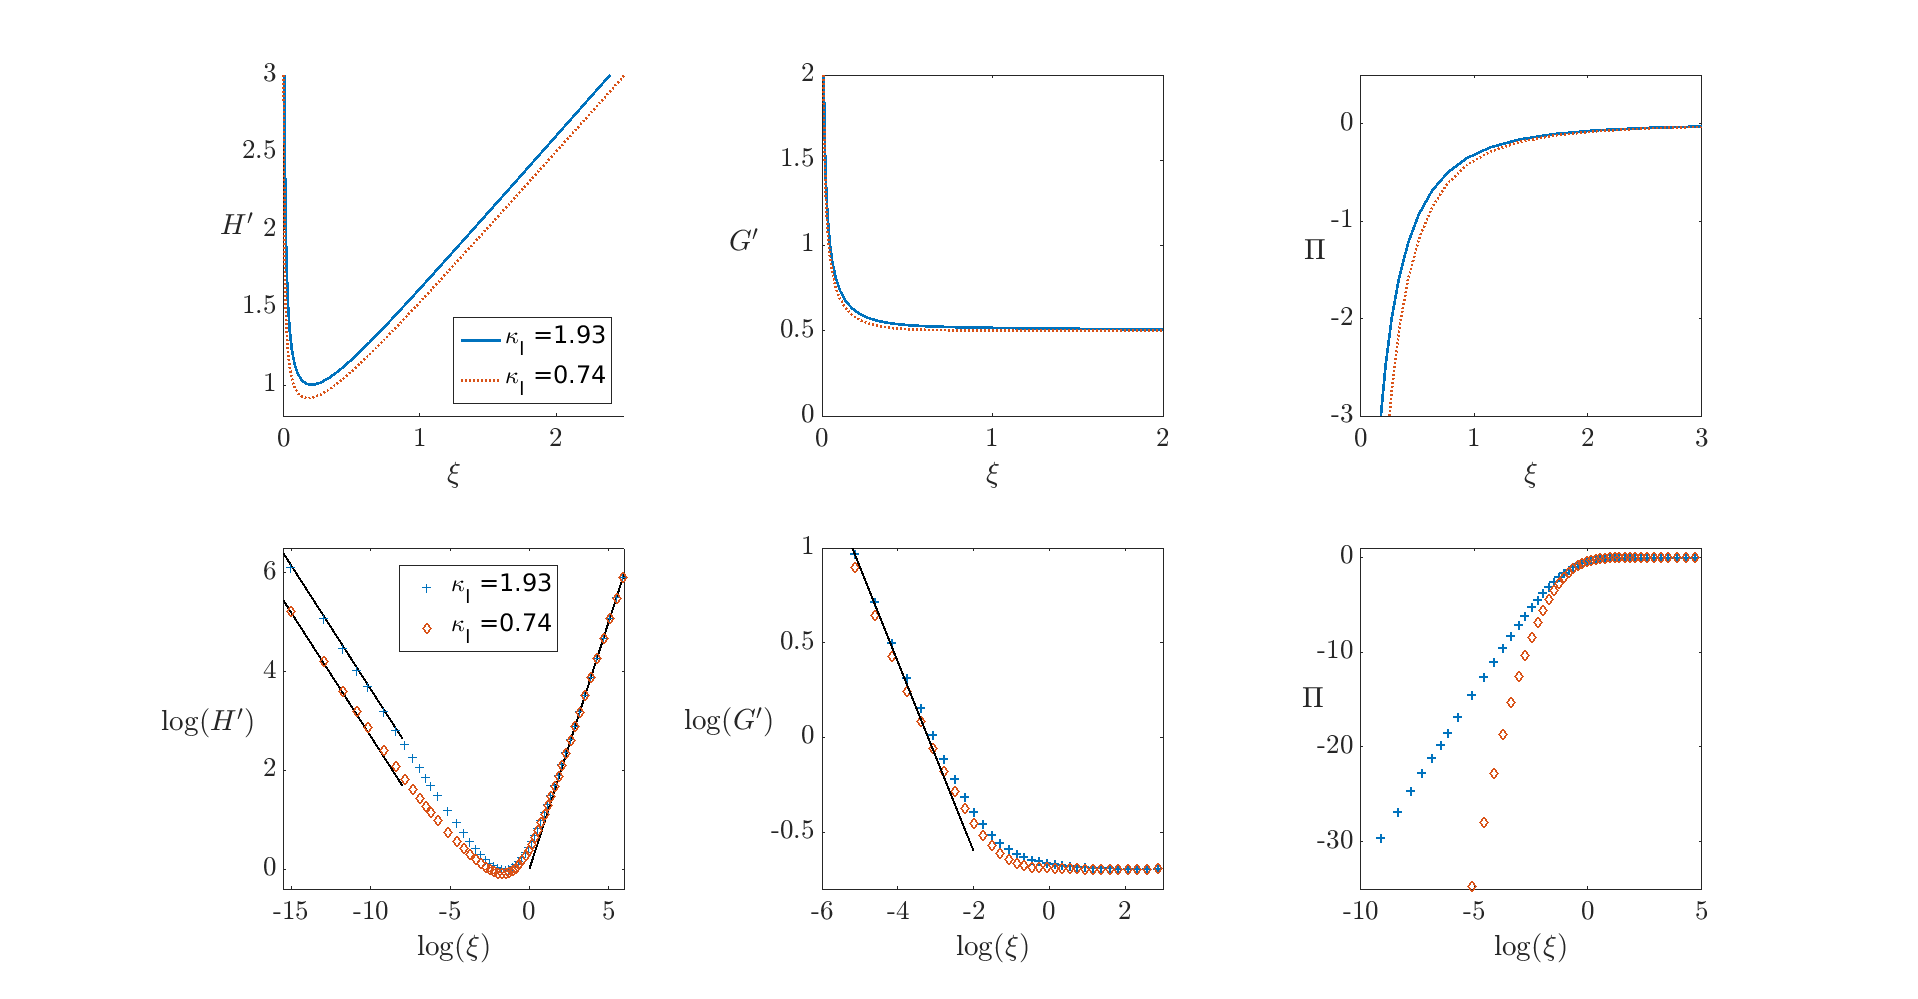
\includegraphics[scale=0.3]{./../../Graphs/hprime-p-x-full.png}}
  \caption{Numerical solutions for two typical $\kappa_I$ values. log-log plots
           are shown for $H'$,$G'$, with solid lines indicating the predicted 
           asymptotics; $\log(H') \approx -\frac{1}{2}\kappa_I \log(\xi)$, 
           $\log(G') \approx -\frac{1}{2} \kappa_{II}\log(\xi)$ near $\xi=0$, 
           and $\log(H') \approx \log(\xi)$, $\log(G') \approx -\log(2)$, as 
           $\xi \to \infty$. Figure produced with $n=465$, $x_n=819$.}
\end{figure}
\begin{figure}
  \centerline{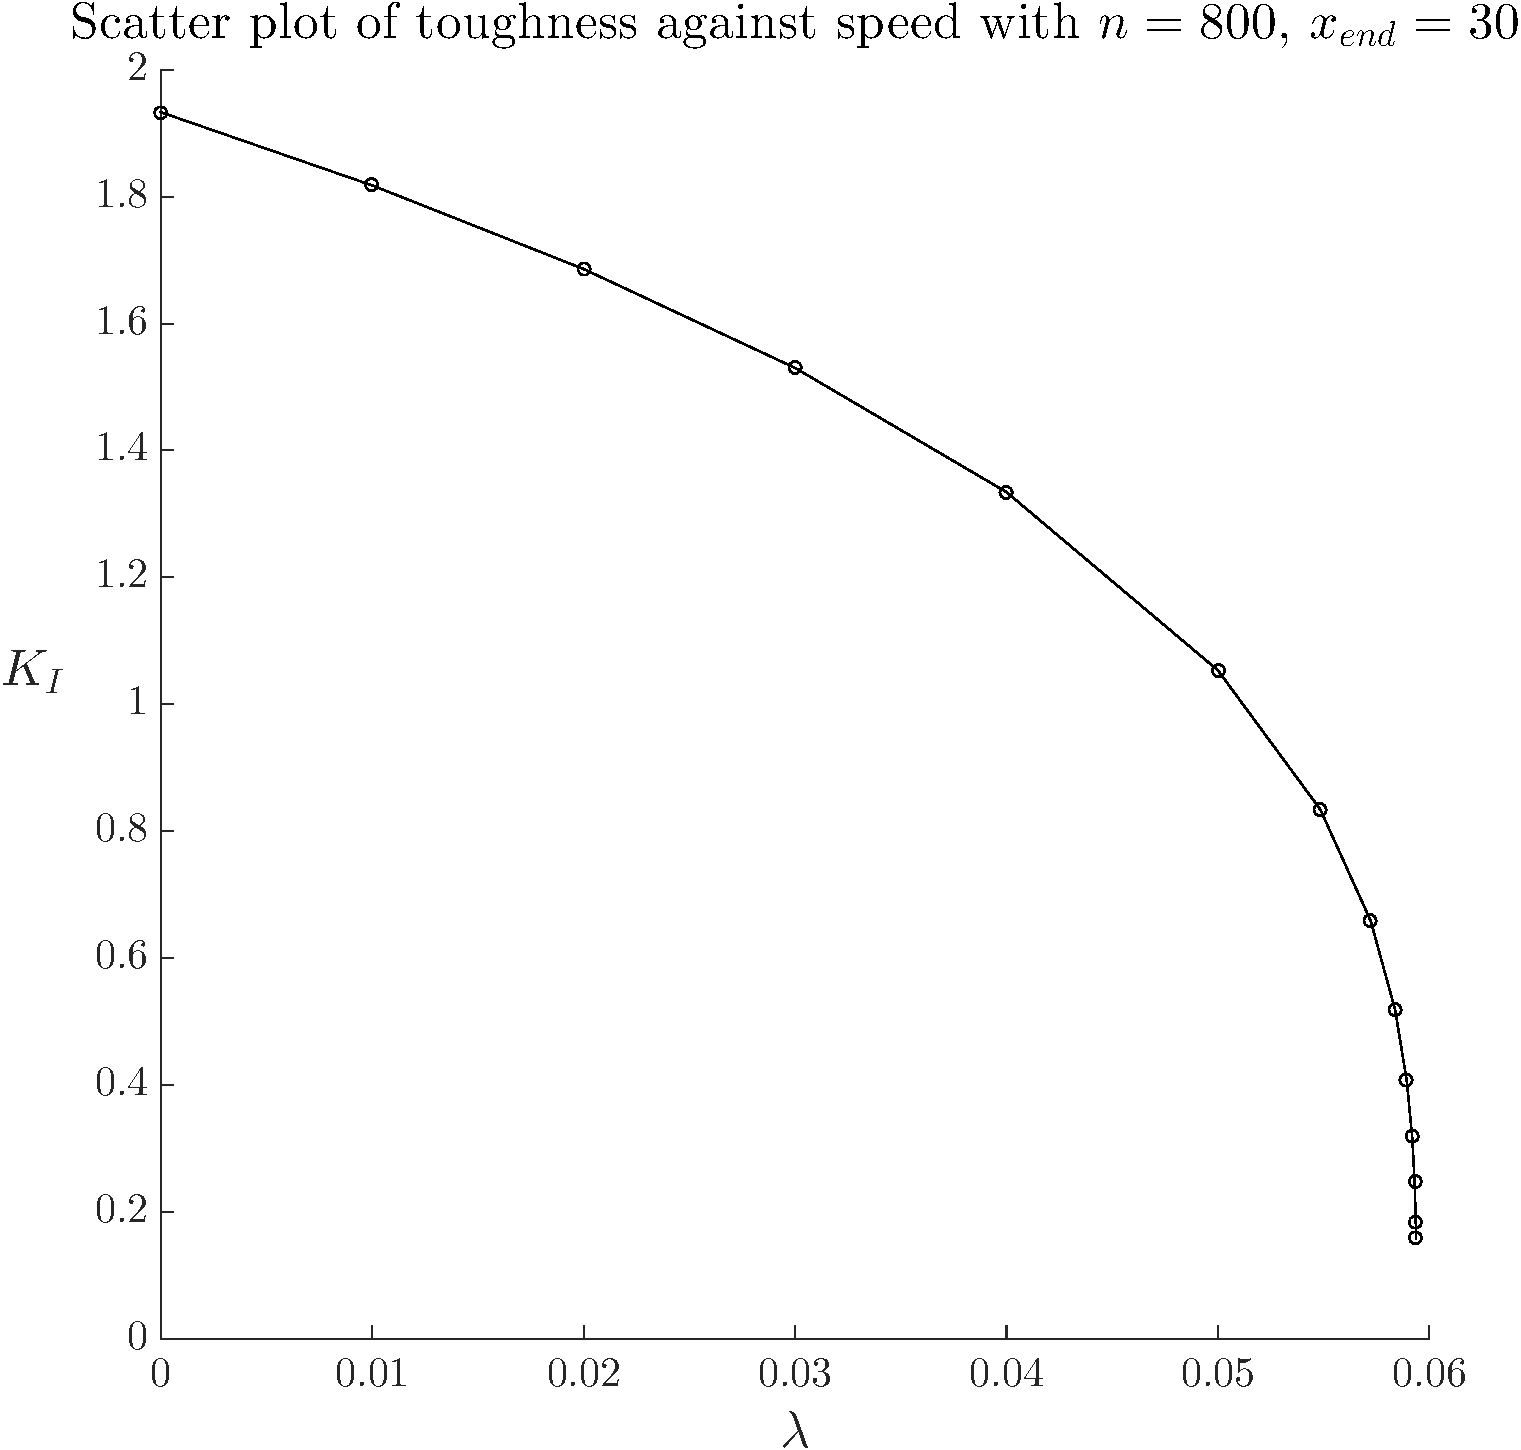
\includegraphics{./../../Graphs/K-lambda.pdf}}
  \caption{Here we vary the parameter $\lambda$ and plot the change in 
           $\kappa_I$. Figure produced with $n=465$, $x_n = 819$.}
\end{figure}
\begin{figure}
  \centerline{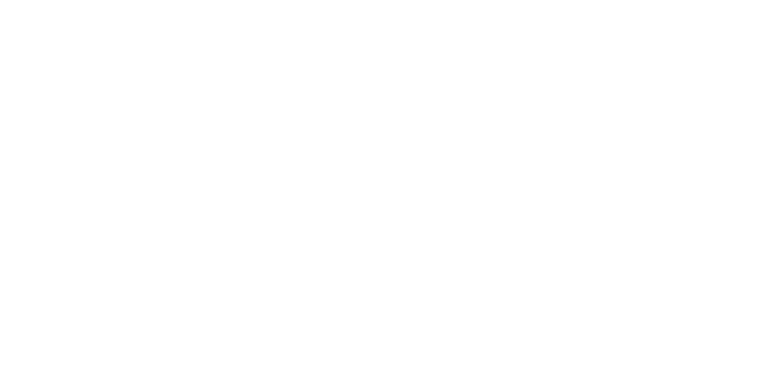
\includegraphics{./../../Graphs/hprime-x.pdf}}
  \caption{As $\kappa_I\to 0$, $H'$ moves from a $\xi^{-1/2}$ singularity
           to a $\xi^{-1/3}$ singularity. We can not calculate $\kappa_I=0$, 
           but the extrapolation to it is shown.}
\end{figure}
\begin{figure}
  \centerline{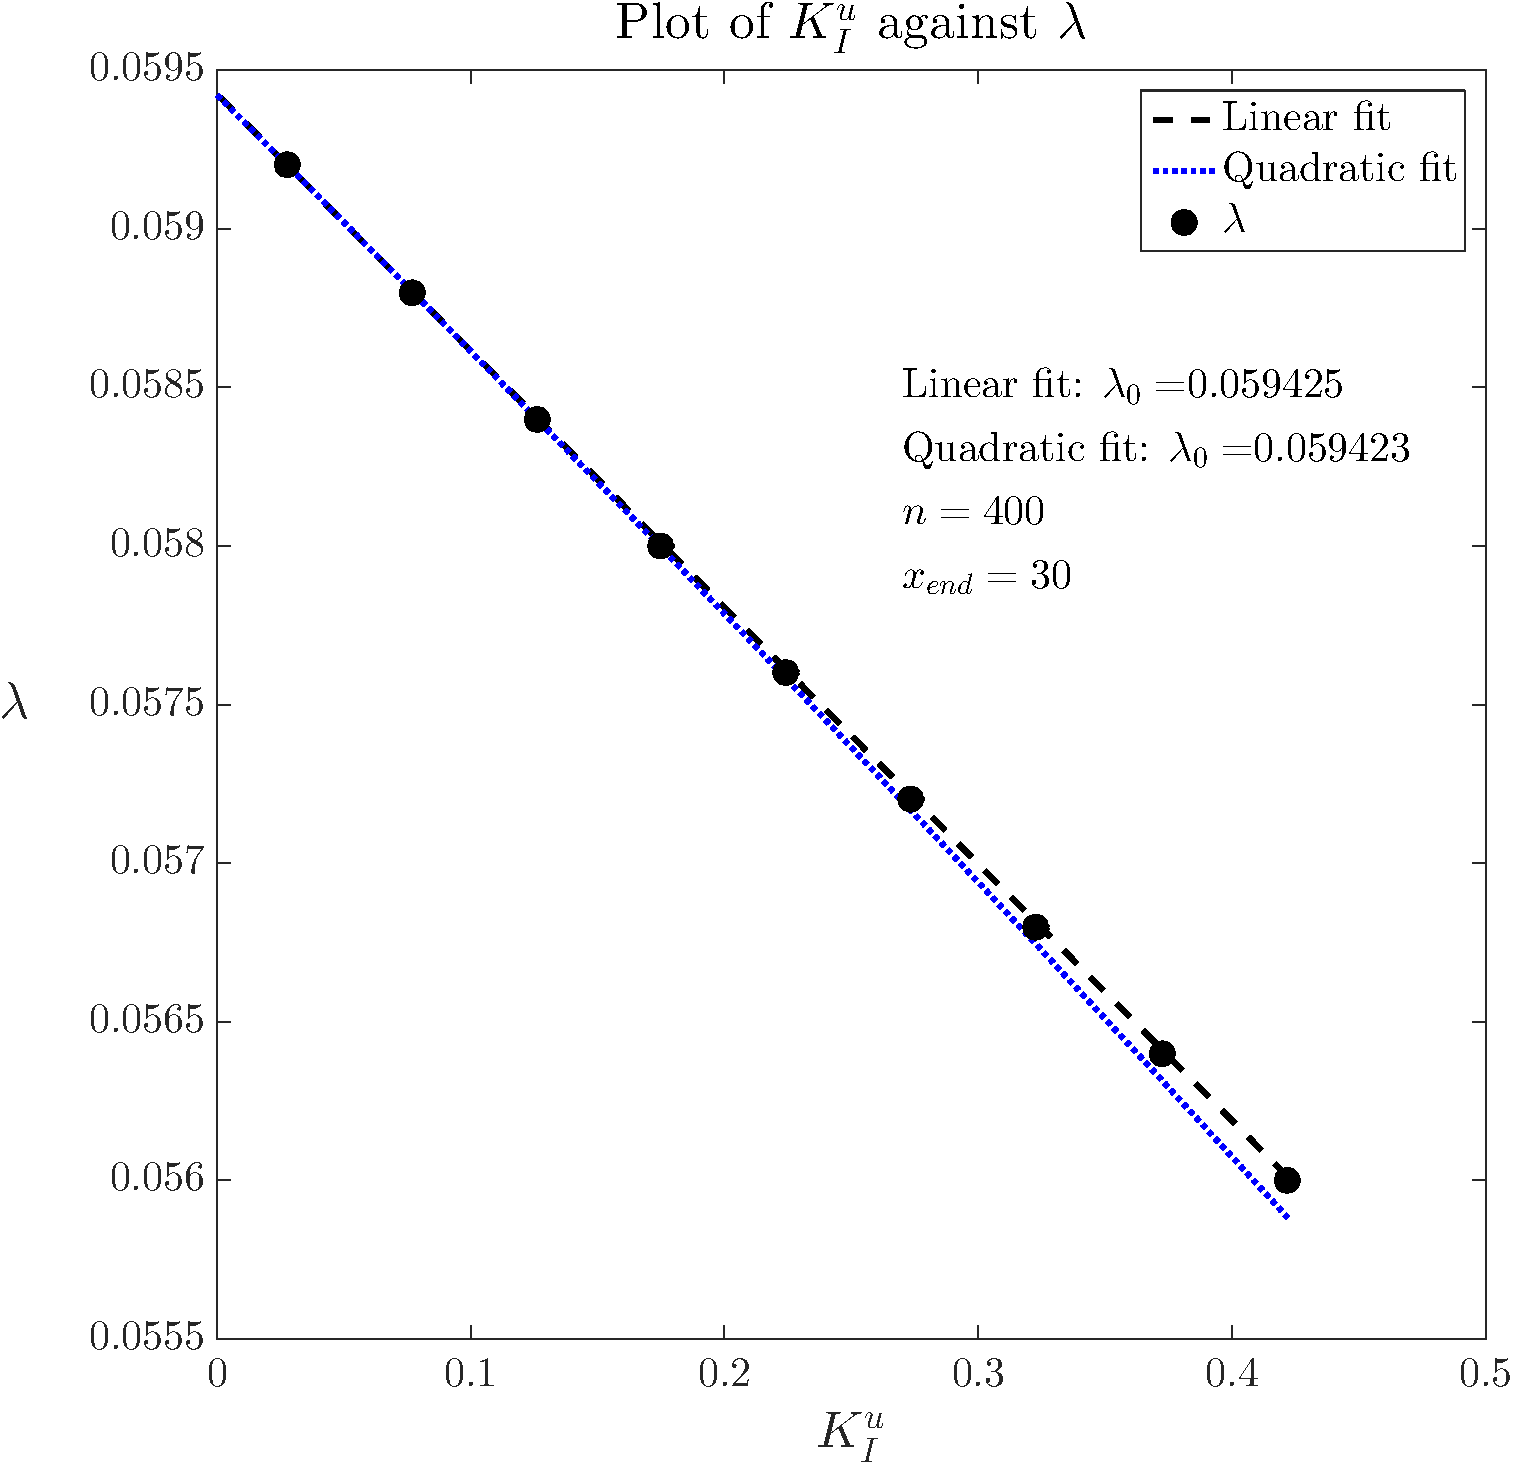
\includegraphics{./../../Graphs/l0.pdf}}
  \caption{A linear fit from the two smallest $\kappa_I$ values is plotted, 
           as is a quadratic fit from the three smallest $\kappa_I$ values.
           They are almost indistiguishable at this scale. 
           The difference between the two extrapolations to $\kappa_I=0$,  
           provides an estimate of the error in calculating $\lambda_0$, 
           (not accounting for the error due to $n$.) }
\end{figure}

Obvious questions to ask at this point are: How are you sure this is the right
answer, what is the effect of $n$,  $\xi_{\mathrm{end}}$? 
In the next graph, we determine the effect of extending $\xi_{\mathrm{end}}$,
by adding on extra points (so maintaining the same resolution near the tip).
There is a satisfactory demonstration of convergence.
\begin{figure}
  \centerline{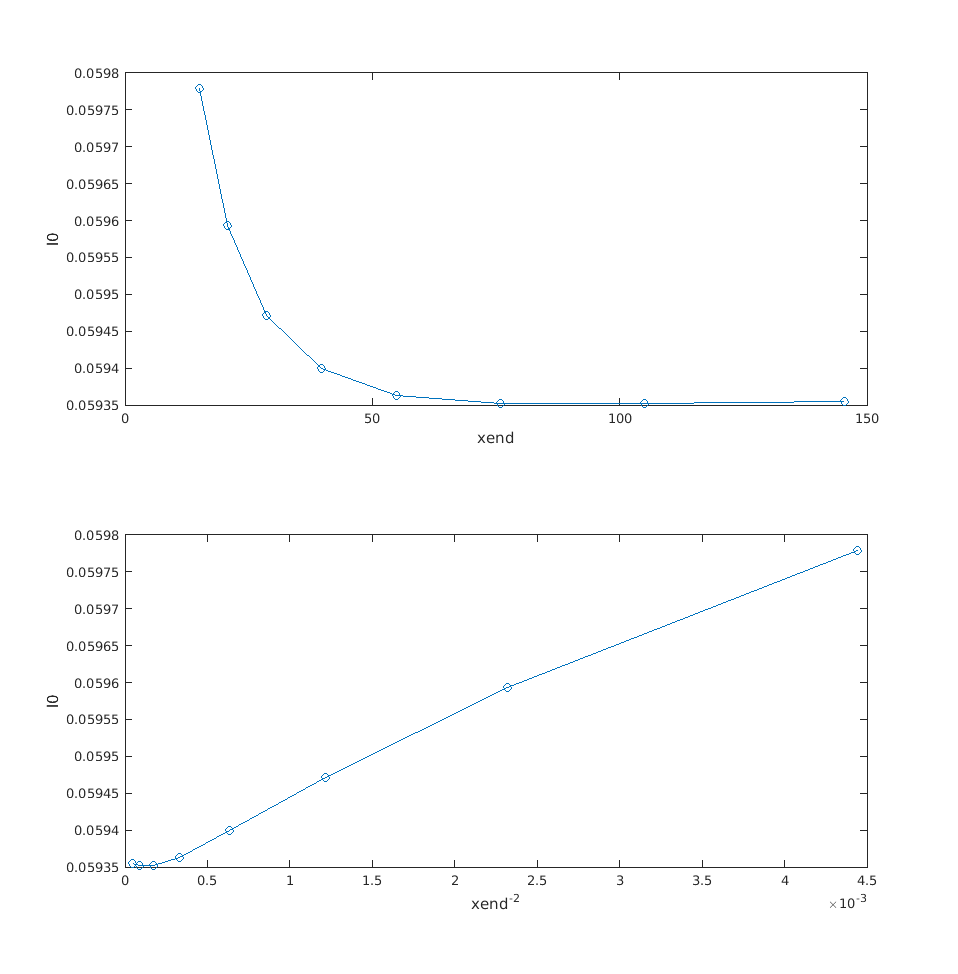
\includegraphics[scale=0.5]{./../../Graphs/xend-march.png}}
  \caption{As we increase $\xi_{n}$, we can estimate the effect of finite 
           truncation. The figure starts with $n=400$, and increases $\xi_n$
           by adding more points until $n=544$.}
\end{figure}

By adding points on in a geometric progression, it becomes quite cheap to
extend out to $\xi_{\mbox{end}} \approx 800$ or so. Once one has done this,
it is apparent that the effect of the tip resolution dominates the effect
of finite truncation, as the following figure shows.

By increasing $n$ (for large $\xi_{\mathrm{end}}$), we have been able to 
determine $\lambda_0$ and $D$
\begin{figure}
  \centerline{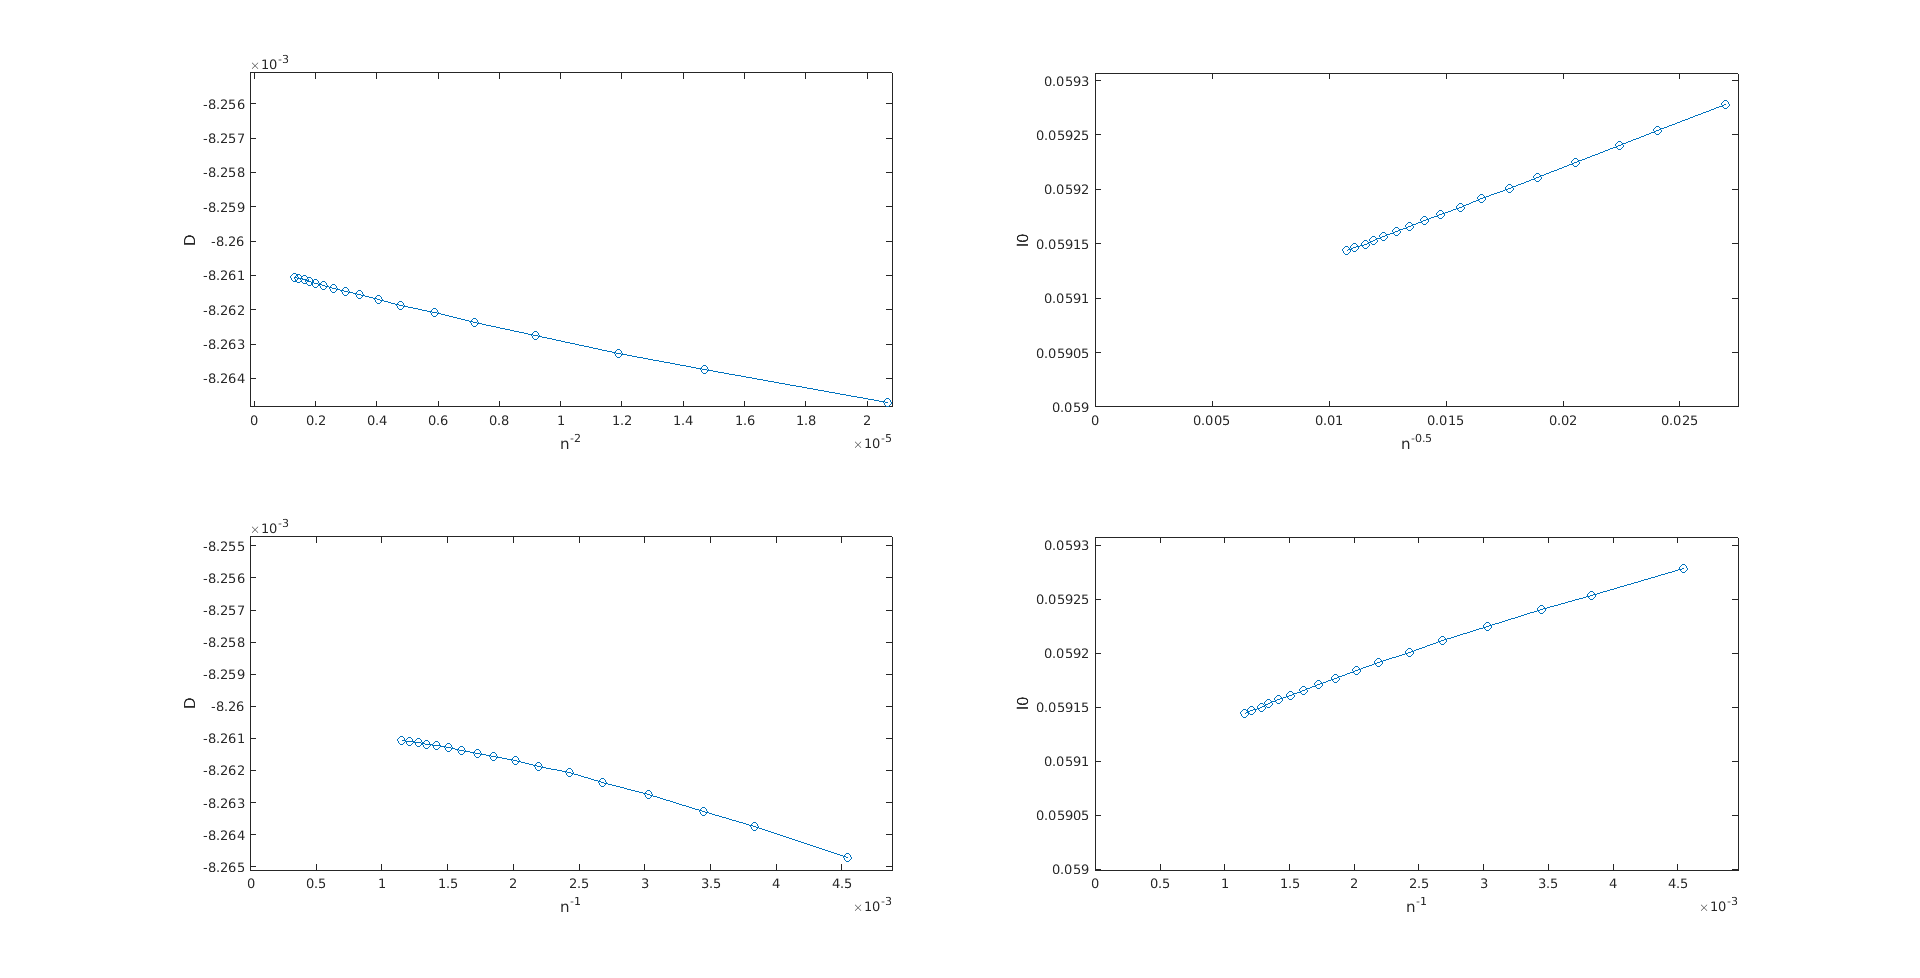
\includegraphics[scale=0.3]{./../../Graphs/l0-D.png}}
  \caption{Our best guess at $\lambda_0$ and $D$, and the approximate error
one can expect in them}
\end{figure}
\subsection{Linear perturbation problem}
We solve the linear perturbation problem. All that we really want to know
is that we see the $\xi^{s-1}$ behaviour that we expect, and we ask what the
intercept of $\tilde{H}_1$ is. It is perhaps worth mentioning the difficulties
in measuring the intercept and perhaps a notion of the sensitivity of the 
result on the estimate provided for $H_0$. Illustrating that is the next
figure 

Then we include the figure that shows convergence with different $n$ values
to something approaching the right answer.
\begin{figure}
 \centerline{
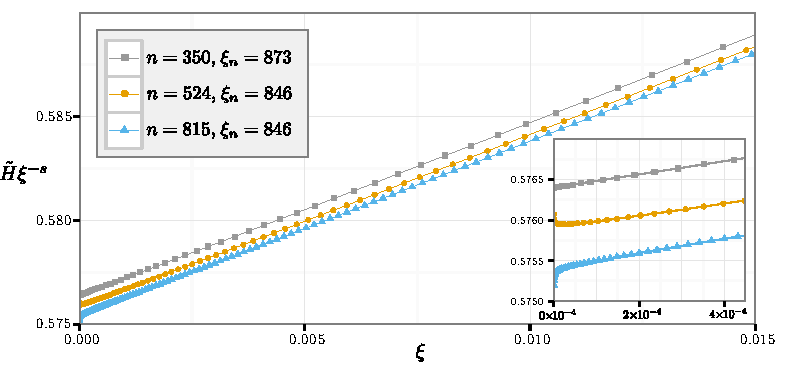
\includegraphics{./../../Graphs/linear-perturbation-plot-edited.pdf}}
  \caption{The numerical solution of the linear perturbation problem for a selection of
           resolutions. Of interest is the value of the intercept, which as shown is dependent
           on the resolution. Also shown is the numerical instability near the tip, due to our 
           difficulty in calculating $H_0$ for $\xi \ll 1$.}
\end{figure}

\subsection{Two tips}
After the linear perturbation problem, we move on to the two tip
problem. Perhaps some graphs that show an outline of the full numerical problem
with non-zero $\kappa_I$ and $\kappa_{II}$, although these are not physical.
\begin{figure}
 \centerline{
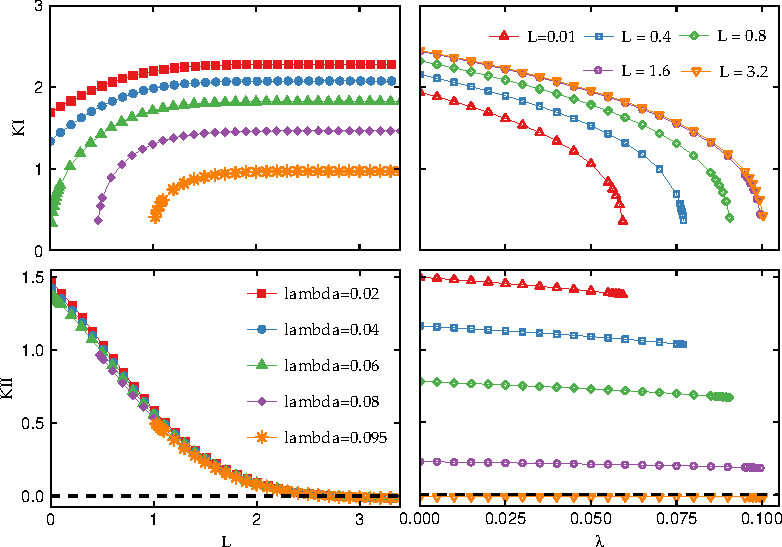
\includegraphics{./../../Graphs/KI-KII-edited.pdf}}
  \caption{Some of the numerical results for the two tip problem. Having 
           $\kappa_{I} \neq 0$ at $\xi =0$ and $L \neq 0$ is unphysical, but
           is what is found numerically. We can recover the physical solution
           by increasing $\lambda$ for fixed $L$ until $\kappa_I =0$.}
\end{figure}

What would be nice, although it doesn't exist yet, is some sort of record of
how we now extrapolate to $\kappa_I=0$. This is certainly a plot that needs to 
be made.
We now move on to the $\kappa_I=0$ set of relations.
\begin{figure}
 \centerline{
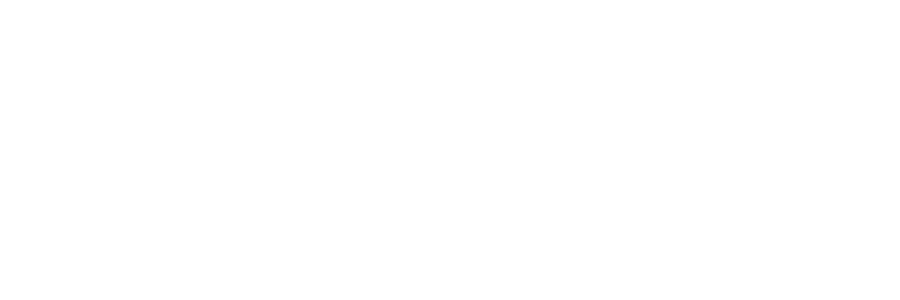
\includegraphics{./../../Graphs/KI-0.pdf}}
  \caption{The results of extrapolating to $\kappa_I = 0$}
\end{figure}


\begin{figure}
 \centerline{
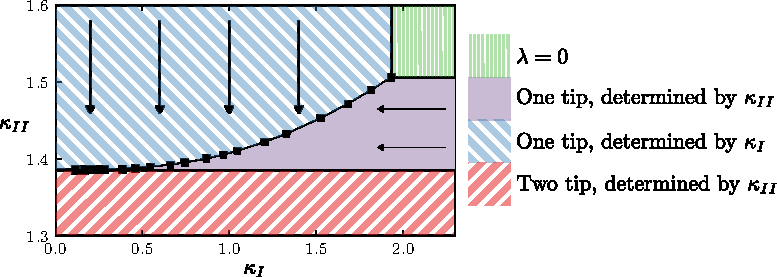
\includegraphics{./../../Graphs/catagory-edited.pdf}}
  \caption{Given values $(\kappa_I,\kappa_{II})$, this graph determines which
           frature regime occurs and so how $\lambda$ and/or $L$ should be 
           calculated. }
\end{figure}
\section{Discussion}
This is where we discuss the figures, possibly include more figures, and draw
the results and conclusions of this paper.

Perhaps the first thing worth mentioning is the somewhat contrived, but pretty
accurate formulae for $\lambda$ in terms of $\kappa_I$. This holds for any 
toughness in the single tip case.
\begin{figure}
 \centerline{
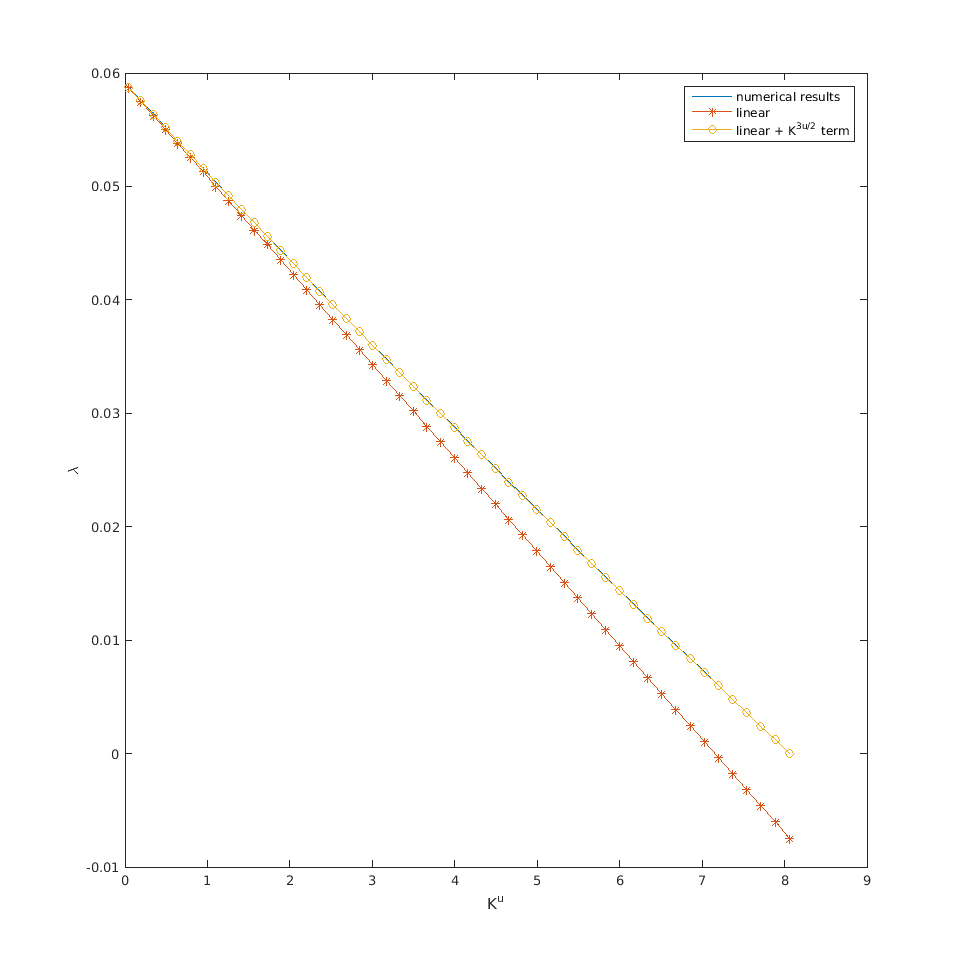
\includegraphics[scale=0.3]{./../../Graphs/overall-fit.png}}
  \caption{The formula valid for all $\kappa_I$}
\end{figure}

Then we could move on to talk about the decoupling between the fluid problem
and the dry fracture problem. Relavent graphs to include would show that
$H$ really doesn't vary much with $\lambda_0$, and that given a reference
$H'$, one can construct $G'$ with relative ease.

\begin{figure}
 \centerline{
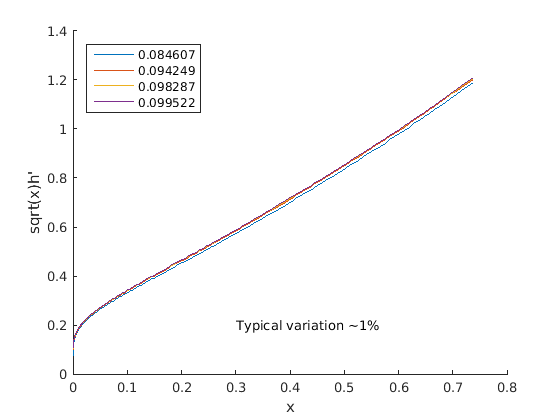
\includegraphics[scale=0.4]{./../../Graphs/hprime-variation.png}}
  \caption{Demonstrating the decoupling of fluid and solid fracture}
\end{figure}
%
\begin{figure}
 \centerline{
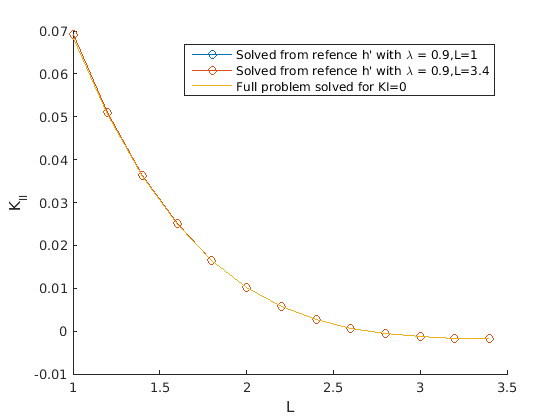
\includegraphics[scale=0.4]{./../../Graphs/fixed-fluid.png}}
  \caption{Reconstructing the full solution given a reference $H'$}
\end{figure}
At this point, I would like to construct another contrived formulae for the
two tip problem. Then I would like to plot a graph of $\kappa_I$ against
$\kappa_{II}$ in the full fluid problem. This provides a guide of when it
is appropriate to take the single tip, and when it is appropriate to take
the double tip. 

\clearpage

\begin{table}
  \begin{center}
\def~{\hphantom{0}}
  \begin{tabular}{lccc}
      $a/d$  & $M=4$   &   $M=8$ & Callan \etal \\[3pt]
       0.1   & 1.56905 & ~~1.56~ & 1.56904\\
       0.3   & 1.50484 & ~~1.504 & 1.50484\\
       0.55  & 1.39128 & ~~1.391 & 1.39131\\
       0.7   & 1.32281 & ~10.322 & 1.32288\\
       0.913 & 1.34479 & 100.351 & 1.35185\\
  \end{tabular}
  \caption{Values of $kd$ at which trapped modes occur when $\rho(\theta)=a$}
  \label{tab:kd}
  \end{center}
\end{table}

\section{Citations and references}
All papers included in the References section must be cited in the article, and vice versa. Citations should be included as, for example ``It has been shown \citep{Rogallo81} that...'' (using the {\verb}\citep} command, part of the natbib package) ``recent work by \citet{Dennis85}...'' (using {\verb}\citet}).
The natbib package can be used to generate citation variations, as shown below.\\
\verb#\citet[pp. 2-4]{Hwang70}#:\\
\citet[pp. 2-4]{Hwang70} \\
\verb#\citep[p. 6]{Worster92}#:\\
\citep[p. 6]{Worster92}\\
\verb#\citep[see][]{Koch83, Lee71, Linton92}#:\\
\citep[see][]{Koch83, Lee71, Linton92}\\
\verb#\citep[see][p. 18]{Martin80}#:\\
\citep[see][p. 18]{Martin80}\\
\verb#\citep{Brownell04,Brownell07,Ursell50,Wijngaarden68,Miller91}#:\\
\citep{Brownell04,Brownell07,Ursell50,Wijngaarden68,Miller91}\\
The References section can either be built from individual \verb#\bibitem# commands, or can be built using BibTex. The BibTex files used to generate the references in this document can be found in the zip file at http://journals.cambridge.org/\linebreak[3]data/\linebreak[3]relatedlink/\linebreak[3]jfm-ifc.zip.\\
Where there are up to ten authors, all authors' names should be given in the reference list. Where there are more than ten authors, only the first name should appear, followed by et al.\\

Acknowledgements should be included at the end of the paper, before the References section or any appendicies, and should be a separate paragraph without a heading. Several anonymous individuals are thanked for contributions to these instructions.

\appendix
\section{}\label{appA}
This appendix contains sample equations in the JFM style. Please refer to the {\LaTeX} source file for examples of how to display such equations in your manuscript.

\begin{equation}
  (\nabla^2+k^2)G_s=(\nabla^2+k^2)G_a=0
  \label{Helm}
\end{equation}

\begin{equation}
  \bnabla\bcdot\boldsymbol{v} = 0,\quad \nabla^{2}P=
    \bnabla\bcdot(\boldsymbol{v}\times \boldsymbol{w}).
\end{equation}

\begin{equation}
  G_s,G_a\sim 1 / (2\upi)\ln r
  \quad \mbox{as\ }\quad r\equiv|P-Q|\rightarrow 0,
  \label{singular}
\end{equation}

\begin{equation}
\left. \begin{array}{ll}  
\displaystyle\frac{\p G_s}{\p y}=0
  \quad \mbox{on\ }\quad y=0,\\[8pt]
\displaystyle  G_a=0
  \quad \mbox{on\ }\quad y=0,
 \end{array}\right\}
  \label{symbc}
\end{equation}


\begin{equation}
  -\frac{1}{2\upi} \int_0^{\infty} \gamma^{-1}[\mathrm exp(-k\gamma|y-\eta|)
   + \mathrm exp(-k\gamma(2d-y-\eta))] \cos k(x-\xi)t\:\mathrm{d} t,
   \qquad 0<y,\quad \eta<d,
\end{equation}

\begin{equation}
  \gamma(t) = \left\{
    \begin{array}{ll}
      -\mathrm{i}(1-t^2)^{1/2}, & t\le 1 \\[2pt]
      (t^2-1)^{1/2},         & t>1.
    \end{array} \right.
\end{equation}

\[
  -\frac{1}{2\upi}
   \pvi B(t)\frac{\cosh k\gamma(d-y)}{\gamma\sinh k\gamma d}
   \cos k(x-\xi)t\:\mathrm{d} t
\]

\begin{equation}
  G = -\frac{1}{4}\mathrm{i} (H_0(kr)+H_0(kr_1))
    - \frac{1}{\upi} \pvi\frac{\mathrm{e}^{-\kgd}}%
    {\gamma\sinh\kgd} \cosh k\gamma(d-y) \cosh k\gamma(d-\eta)
\end{equation}

Note that when equations are included in definitions, it may be suitable to render them in line, rather than in the equation environment: $\boldsymbol{n}_q=(-y^{\prime}(\theta),
x^{\prime}(\theta))/w(\theta)$.
Now $G_a=\squart Y_0(kr)+\Gat$ where
$r=\{[x(\theta)-x(\psi)]^2 + [y(\theta)-y(\psi)]^2\}^{1/2}$ and $\Gat$ is
regular as $kr\ttz$. However, any fractions displayed like this, other than $\thalf$ or $\squart$, must be written on the line, and not stacked (ie 1/3).
 
\begin{eqnarray}
  \ndq\left(\frac{1}{4} Y_0(kr)\right) & \sim &
    \frac{1}{4\upi w^3(\theta)}
    [x^{\prime\prime}(\theta)y^{\prime}(\theta)-
    y^{\prime\prime}(\theta)x^{\prime}(\theta)] \nonumber\\
  & = & \frac{1}{4\upi w^3(\theta)}
    [\rho^{\prime}(\theta)\rho^{\prime\prime}(\theta)
    - \rho^2(\theta)-2\rho^{\prime 2}(\theta)]
    \quad \mbox{as\ }\quad kr\ttz . \label{inteqpt}
\end{eqnarray}

\begin{equation}
  \frac{1}{2}\phi_i = \frac{\upi}{M} \sumjm\phi_j K_{ij}^a w_j,
  \qquad i=1,\,\ldots,\,M,
\end{equation}
where
\begin{equation}
  K_{ij}^a = \left\{
    \begin{array}{ll}
      \p G_a(\theta_i,\theta_j)/\p n_q, & i\neq j \\[2pt]
      \p\Gat(\theta_i,\theta_i)/\p n_q
      + [\rho_i^{\prime}\rho_i^{\prime\prime}-\rho_i^2-2\rho_i^{\prime 2}]
      / 4\upi w_i^3, & i=j.
  \end{array} \right.
\end{equation}


\refstepcounter{equation}
$$
  \rho_l = \lim_{\zeta \rightarrow Z^-_l(x)} \rho(x,\zeta), \quad
  \rho_{u} = \lim_{\zeta \rightarrow Z^{+}_u(x)} \rho(x,\zeta)
  \eqno{(\theequation{\mathit{a},\mathit{b}})}\label{eq35}
$$

\begin{equation}
  (\rho(x,\zeta),\phi_{\zeta\zeta}(x,\zeta))=(\rho_0,N_0)
  \quad \mbox{for}\quad Z_l(x) < \zeta < Z_u(x).
\end{equation}


\begin{subeqnarray}
  \tau_{ij} & = &
    (\overline{\overline{u}_i \overline{u}_j}
    - \overline{u}_i\overline{u}_j)
    + (\overline{\overline{u}_iu^{SGS}_j
    + u^{SGS}_i\overline{u}_j})
    + \overline{u^{SGS}_iu^{SGS}_j},\\[3pt]
  \tau^\theta_j & = &
    (\overline{\overline{u}_j\overline{\theta}}
    - \overline{u}_j \overline{\theta})
    + (\overline{\overline{u}_j\theta^{SGS}
    + u^{SGS}_j \overline{\theta}})
    + \overline{u^{SGS}_j\theta^{SGS}}.
\end{subeqnarray}

\begin{equation}
\setlength{\arraycolsep}{0pt}
\renewcommand{\arraystretch}{1.3}
\slsQ_C = \left[
\begin{array}{ccccc}
  -\omega^{-2}V'_w  &  -(\alpha^t\omega)^{-1}  &  0  &  0  &  0  \\
  \displaystyle
  \frac{\beta}{\alpha\omega^2}V'_w  &  0  &  0  &  0  &  \mathrm{i}\omega^{-1} \\
  \mathrm{i}\omega^{-1}  &  0  &  0  &  0  &  0  \\
  \displaystyle
  \mathrm{i} R^{-1}_{\delta}(\alpha^t+\omega^{-1}V''_w)  &  0
    & -(\mathrm{i}\alpha^tR_\delta)^{-1}  &  0  &  0  \\
  \displaystyle
  \frac{\mathrm{i}\beta}{\alpha\omega}R^{-1}_\delta V''_w  &  0  &  0
    &  0  & 0 \\
  (\mathrm{i}\alpha^t)^{-1}V'_w  &  (3R^{-1}_{\delta}+c^t(\mathrm{i}\alpha^t)^{-1})
    &  0  &  -(\alpha^t)^{-2}R^{-1}_{\delta}  &  0  \\
\end{array}  \right] .
\label{defQc}
\end{equation}

\begin{equation}
\etb^t = \skew2\hat{\etb}^t \exp [\mathrm{i} (\alpha^tx^t_1-\omega t)],
\end{equation}
where $\skew2\hat{\etb}^t=\boldsymbol{b}\exp (\mathrm{i}\gamma x^t_3)$. 
\begin{equation}
\mbox{Det}[\rho\omega^2\delta_{ps}-C^t_{pqrs}k^t_qk^t_r]=0,
\end{equation}

\begin{equation}
 \langle k^t_1,k^t_2,k^t_3\rangle = \langle
\alpha^t,0,\gamma\rangle  
\end{equation}

\begin{equation}
\boldsymbol{f}(\theta,\psi) = (g(\psi)\cos \theta,g(\psi) \sin \theta,f(\psi)).
\label{eq41}
\end{equation}

\begin{eqnarray}
f(\psi_1) = \frac{3b}{\upi[2(a+b \cos \psi_1)]^{{3}/{2}}}
  \int^{2\upi}_0 \frac{(\sin \psi_1 - \sin \psi)(a+b \cos \psi)^{1/2}}%
  {[1 - \cos (\psi_1 - \psi)](2+\alpha)^{1/2}}\mathrm{d}x,
\label{eq42}
\end{eqnarray}
\begin{eqnarray}
g(\psi_1) & = & \frac{3}{\upi[2(a+b \cos \psi_1)]^{{3}/{2}}}
  \int^{2\upi}_0 \left(\frac{a+b \cos \psi}{2+\alpha}\right)^{1/2}
  \left\{ \astrut f(\psi)[(\cos \psi_1 - b \beta_1)S + \beta_1P]
  \right. \nonumber\\
&& \mbox{}\times \frac{\sin \psi_1 - \sin \psi}{1-\cos(\psi_1 - \psi)}
  + g(\psi) \left[\left(2+\alpha - \frac{(\sin \psi_1 - \sin \psi)^2}
  {1- \cos (\psi - \psi_1)} - b^2 \gamma \right) S \right.\nonumber\\
&& \left.\left.\mbox{} + \left( b^2 \cos \psi_1\gamma -
  \frac{a}{b}\alpha \right) F(\frac{1}{2}\upi, \delta) - (2+\alpha)
  \cos\psi_1 E(\frac{1}{2}\upi, \delta)\right] \astrut\right\} \mathrm{d} \psi,
\label{eq43}
\end{eqnarray}
\begin{equation}
\alpha = \alpha(\psi,\psi_1) = \frac{b^2[1-\cos(\psi-\psi_1)]}%
  {(a+b\cos\psi) (a+b\cos\psi_1)},
  \quad
  \beta - \beta(\psi,\psi_1) = \frac{1-\cos(\psi-\psi_1)}{a+b\cos\psi}.
\end{equation}


\begin{equation}
\left. \begin{array}{l}
\displaystyle
H(0) = \frac{\epsilon \overline{C}_v}{\tilde{v}^{{1}/{2}}_T
(1- \beta)},\quad H'(0) = -1+\epsilon^{{2}/{3}} \overline{C}_u
+ \epsilon \skew5\hat{C}_u'; \\[16pt]
\displaystyle
H''(0) = \frac{\epsilon u^2_{\ast}}{\tilde{v}^{{1}/{2}}
_T u^2_P},\quad H' (\infty) = 0.
\end{array} \right\}
\end{equation}

\begin{lemma}
Let $f(z)$ be a trial \citet[][pp.~231--232]{Batchelor59} function defined on $[0,1]$.  Let $\varLambda_1$ denote
the ground-state eigenvalue for $-\mathrm{d}^2g/\mathrm{d} z^2=\varLambda g$,
where $g$ must satisfy $\pm\mathrm{d} g/\mathrm{d} z+\alpha g=0$ at $z=0,1$
for some non-negative constant~$\alpha$.  Then for any $f$ that is not
identically zero we have
\begin{equation}
\frac{\displaystyle
  \alpha(f^2(0)+f^2(1)) + \int_0^1 \left(
  \frac{\mathrm{d} f}{\mathrm{d} z} \right)^2 \mathrm{d} z}%
  {\displaystyle \int_0^1 f^2\mathrm{d} z}
\ge \varLambda_1 \ge
\left( \frac{-\alpha+(\alpha^2+8\upi^2\alpha)^{1/2}}{4\upi} \right)^2.
\end{equation}
\end{lemma}

\begin{corollary}
Any non-zero trial function $f$ which satisfies the boundary condition
$f(0)=f(1)=0$ always satisfies
\begin{equation}
  \int_0^1 \left( \frac{\mathrm{d} f}{\mathrm{d} z} \right)^2 \mathrm{d} z.
\end{equation}
\end{corollary}

\bibliographystyle{jfm}
% Note the spaces between the initials
\bibliography{elastic-fracture}

\end{document}
